\begin{enumerate} 
    \item  \textbf{Enzyme cứng hay mềm ?}\\
    \begin{enumerate}[label=\textbf{\alph*,}]\itemsep0em
        \item Giả sử abzyme biến dạng một lượng $x_1$ và cơ chất biến dạng một lượng $x_2$. Từ trạng thái chuyển tiếp như hình vẽ trong đề bài, cơ chất liên kết với vùng hoạt động, do đó:
        \begin{equation} \label{eq1_enzyme}
            a+x_1=2d-x_2.
        \end{equation}
        Mặt khác, ta có định luật 3 Newton cho cân bằng lực ở vùng hoạt động:
        \begin{equation} \label{eq2_enzyme}
            k_e x_1 = k_s x_2.
        \end{equation}
        Từ phương trình (\ref{eq1_enzyme}) và phương trình (\ref{eq2_enzyme}), ta suy ra $x_1$ và $x_2$:
        \begin{equation} \label{eq3_enzyme}
        \begin{split}
            x_1=\dfrac{k_s}{k_e+k_s}(2d-a),\\
            x_2=\dfrac{k_e}{k_e+k_s}(2d-a).
        \end{split}
        \end{equation}
        Năng lượng cung cấp cho enzyme gây ra biến dạng của enzyme là:
        \begin{equation} \label{eq4_enzyme}
            E_e=\dfrac{1}{2}k_e x_1^2 =  \dfrac{k_e k_s^2}{2(k_e+k_s)^2}(2d-a)^2. 
        \end{equation}
        Năng lượng cung cấp cho cơ chất gây ra biến dạng của cơ chất là:
        \begin{equation} \label{eq5_enzyme}
            E_s=\dfrac{1}{2}k_s x_2^2 =  \dfrac{k_s k_e^2}{2(k_e+k_s)^2}(2d-a)^2. 
        \end{equation}
    \item Lấy phương trình (\ref{eq4_enzyme}) chia cho phương trình (\ref{eq5_enzyme}), ta thu được liên hệ về năng lượng:
    \begin{equation} \label{eq6_enzyme}
        \dfrac{E_e}{E_s}=\dfrac{k_s}{k_e}.
    \end{equation}
    Như ta đã biết, một enzyme xúc tác càng hiệu quả sẽ tiêu tốn càng ít năng lượng cho việc biến dạng chính nó, hay chính là $E_e \ll E_s$, tương đương với $k_e \gg k_s$. Do đó, một enzyme hoạt động hiệu quả sẽ phải thật "cứng" để phần lớn năng lượng được sử dụng vào biến dạng của cơ chất, từ đó thúc đẩy phản ứng hoá học.\\
    \textit{Trong mô hình này, ta xét abzyme do abzyme chỉ dùng tương tác van der Waals, các enzyme tự nhiên sử dụng cả liên kết cộng hoá trị nên "cứng" hơn nhiều abzyme, do đó mà khả năng xúc tác phản ứng cũng mạnh hơn nhiều lần.}
    \end{enumerate}
    \item \textbf{Bỏ qua động năng?}\\
    \begin{enumerate}[label=\textbf{\alph*,}]\itemsep0em
        \item Phương trình động lực học:
        \begin{equation} \label{eq7_enzyme}
        \begin{split}
            m\dfrac{d^2 x}{dt^2}&=F_{\text{ela}}\\
            \rho V \dfrac{d^2 x}{dt^2}&= - \dfrac{ES}{D}x \\
            \dfrac{d^2 x}{dt^2}+&\dfrac{E}{\rho D^2}x=0.    
        \end{split}
        \end{equation}
        Đặt $\dfrac{E}{\rho D^2}=\omega_0^2$, phương trình (\ref{eq7_enzyme}) trở thành:
        \begin{equation} \label{eq8_enzyme}
            \dfrac{d^2 x}{dt^2}+\omega_0^2 x=0.
        \end{equation}
        Chu kỳ dao động của enzyme:
        \begin{equation} \label{eq9_enzyme}
            T_0=\dfrac{2\pi}{\omega_0}=2\pi \sqrt{\dfrac{\rho D^2}{E}}=2.51 \times 10^{-11} \ \si{s}.
        \end{equation}
        \item 
        \begin{enumerate}
            \item Ta có phương trình động lực học như sau:
        \begin{equation} \label{eq10_enzyme}
        \begin{split}
            m\dfrac{d^2 x}{dt^2} &=F_{\text{vis}}+F_{\text{ela}}\\
            \rho V \dfrac{d^2 x}{dt^2} &=-10 \eta D \dfrac{dx}{dt} - \dfrac{ES}{D}x \\
            \dfrac{d^2 x}{dt^2}+ &\dfrac{10\eta }{\rho D^2}\dfrac{dx}{dt}+\dfrac{E}{\rho D^2}x=0.
        \end{split}
        \end{equation}
        Đặt $\dfrac{10\eta }{\rho D^2}=2\beta$, phương trình (\ref{eq10_enzyme}) trở thành:
        \begin{equation} \label{eq11_enzyme}
            \dfrac{d^2 x}{dt^2}+2\beta\dfrac{dx}{dt}+\omega_0^2 x=0.
        \end{equation}
        Trong đó:
        \begin{equation} \label{eq12_enzyme}
            \beta = \dfrac{5\eta}{\rho D^2}=3.125\times 10^{11} \ \si{s^{-1}}, \quad \omega_0=\sqrt{\dfrac{E}{\rho D^2}}=2.5\times 10^{11}\ \si{s^{-1}}.
        \end{equation}
        Phương trình vi phân (\ref{eq10_enzyme}) có nghiệm là:
        \begin{equation} \label{eq13_enzyme}
            x(t)=Ae^{\lambda_1t}+Be^{\lambda_2t}.
        \end{equation}
        Trong đó:
        \begin{align} \label{eq14_enzyme}
            \lambda_1&=-\beta+\sqrt{\beta^2-\omega_0^2}=-1.25\times 10^{11} \ \si{s^{-1}},\\
            \label{eq15_enzyme}
            \lambda_2&=-\beta-\sqrt{\beta^2-\omega_0^2}=-5\times 10^{11} \ \si{s^{-1}}.
        \end{align}
        Tại $t=0$, $x(0)=x_0$ và $v(0)=x'(0)=0$, suy ra $A=\dfrac{\lambda_2 x_0}{\lambda_2-\lambda_1}=\dfrac{4}{3} x_0$ và $B=\dfrac{\lambda_1 x_0}{\lambda_1-\lambda_2}=-\dfrac{1}{3} x_0$.\\
        Nghiệm của phương trình vi phân (\ref{eq10_enzyme}) có thể viết lại thành:
        \begin{equation} \label{eq16_enzyme}
            x(t)=x_0\left(\dfrac{4}{3}e^{\lambda_1t}-\dfrac{1}{3}e^{\lambda_2t}\right).
        \end{equation}
        Trong đó $\lambda_1=-1.25\times 10^{11} \ \si{s^{-1}}$ và $\lambda_2=-5\times 10^{11} \ \si{s^{-1}}$.
    \begin{figure}[htp]
    \centering
    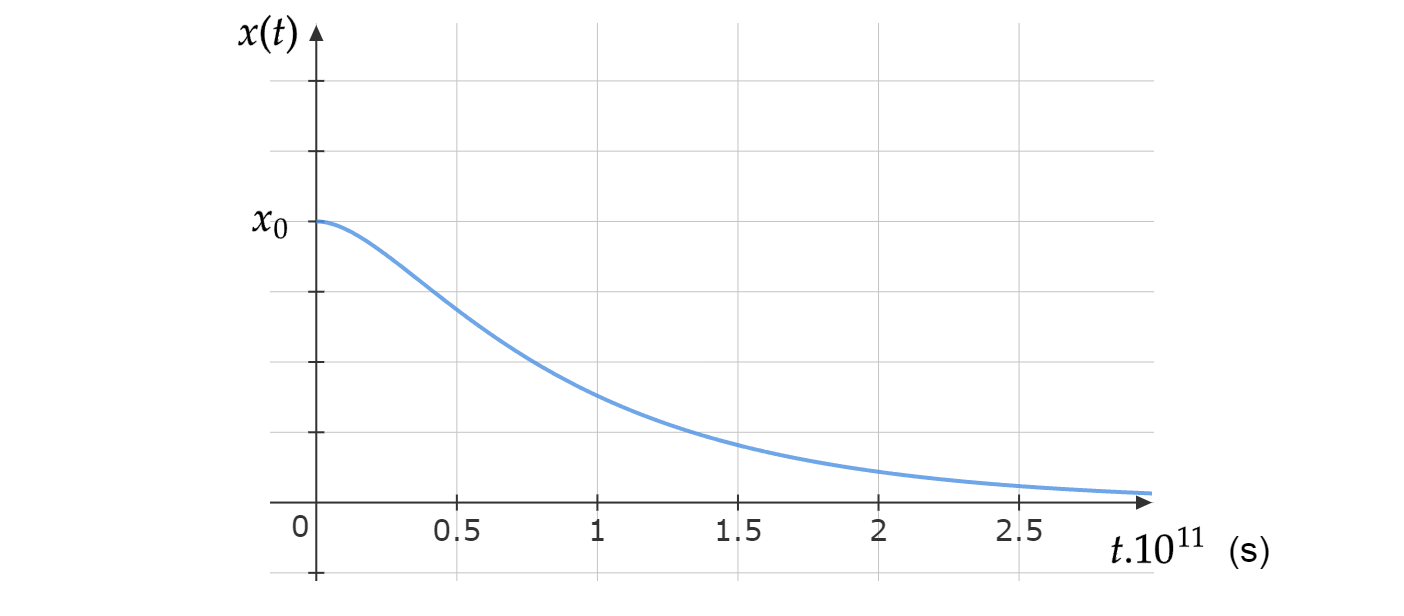
\includegraphics[scale=.27
        ]{Problem_5/image/3.png}
    \caption{Đồ thị $x(t)$.}
    \end{figure}
        \item Tại $t=T_0$, tỉ lệ giữa li độ $x$ và li độ $x_0$ ở thời điểm ban đầu:
        \begin{equation} \label{eq17_enzyme}
            N_1=\dfrac{x(T_0)}{x_0}=\dfrac{4}{3}e^{\lambda_1T_0}-\dfrac{1}{3}e^{\lambda_2T_0} \approx 5.78 \times 10^{-2}.
        \end{equation}
        Tại $t=2T_0$, tỉ lệ giữa li độ $x$ và li độ $x_0$ ở thời điểm ban đầu:
        \begin{equation} \label{eq18_enzyme}
            N_2=\dfrac{x(2T_0)}{x_0}=\dfrac{4}{3}e^{2\lambda_1T_0}-\dfrac{1}{3}e^{2\lambda_2T_0} \approx 2.51 \times 10^{-3}.
        \end{equation}
        
        \textit{Nhận xét: Ta thấy rằng động năng của enzyme bị phân tán và chuyển hoá thành nhiệt quá nhanh (thực tế là trước khi nó có thể được sử dụng trong quá trình xúc tác của enzyme). Quá trình dao động của enzyme hầu như không xảy ra hoặc bị tắt rất nhanh khi chúng ở trong nước (chưa kể đến môi trường nhớt hơn như màng). Do đó trong quá trình xúc tác của enzyme, ta bỏ qua động năng và coi enzyme tĩnh hoặc gần tĩnh.
        \newpage
        Qua bài tập này ta kết luận được hai tính chất rất đặc biệt của enzyme:
        \begin{enumerate}
            \item Năng lượng được cung cấp không phải để thay đổi cấu trúc enzyme mà phần lớn để đưa cơ chất vào enzyme và đưa nó vào trạng thái chuyển tiếp. Do đó vùng hoạt động của enzyme phải là cấu trúc cứng.
            \item Động năng không dùng trong quá trình xúc tác vì nó tiêu tán ra môi trường quá nhanh. Do đó có thể coi các mô hình là tĩnh hoặc gần tĩnh.
        \end{enumerate}}
        \end{enumerate}
    \end{enumerate}
\end{enumerate}

\textbf{Biểu điểm}
\begin{center}
\begin{tabular}{|>{\centering\arraybackslash}m{1cm}|>{\raggedright\arraybackslash}m{14cm}| >{\centering\arraybackslash}m{1cm}|}
    \hline
    \textbf{Phần} & \textbf{Nội dung} & \textbf{Điểm} \\
    \hline
    \textbf{1a} & Viết biểu thức cho $x_1$ và $x_2$ theo $k_e$, $k_s$, $d$ và $a$ (\ref{eq3_enzyme}) & $0.50$ \\
    \cline{2-3}
    &  Viết biểu thức cho $E_e$ theo $k_e$, $k_s$, $d$ và $a$ (\ref{eq4_enzyme}) & $0.25$ \\
    \cline{2-3}
    &  Viết biểu thức cho $E_s$ theo $k_e$, $k_s$, $d$ và $a$ (\ref{eq5_enzyme}) & $0.25$ \\
    \hline
    \textbf{1b} & Lập luận và kết luận & $0.25$ \\
    \hline
    \textbf{2a} & Dẫn ra phương trình vi phân (\ref{eq8_enzyme}) & $0.25$ \\
    \cline{2-3}
    & Tính được chu kỳ dao động $T$ (\ref{eq9_enzyme}) & $0.25$ \\
    \hline
    \textbf{2b.i} & Dẫn ra phương trình vi phân (\ref{eq10_enzyme}) & $0.25$ \\
    \cline{2-3}
    & Viết biểu thức $x(t)$ và các hệ số (\ref{eq16_enzyme}) & $1.25$ \\
    \hline
    \textbf{2b.ii} & Tính được tỉ lệ giữa li độ $x$ và $x_0$ tại thời điểm $t=T_0$ (\ref{eq17_enzyme}) & $0.25$ \\
    \cline{2-3}
    & Tính được tỉ lệ giữa li độ $x$ và $x_0$ tại thời điểm $t=2T_0$ (\ref{eq18_enzyme}) & $0.25$ \\
    \cline{2-3}
    & Lập luận và kết luận & $0.25$ \\
    \hline
\end{tabular}
\end{center}

%% Reference %%
\bibliographystyle{plain}
\begin{thebibliography}{}
\bibitem{bandaria2008} Jigar N. Bandaria, Samrat Dutta, Sarah E. Hill, Amnon Kohen, Christopher M. Cheatum (2008), \textit{Fast Enzyme Dynamics at the Active Site of Formate Dehydrogenase}, Journal of the American Chemical Society, 130(1), 22–23.           
\bibitem{giaotrinh} Nguyễn Thế Toàn, Nguyễn Hoạ Mi (2021), \textit{Giáo trình Vật lý Sinh học của Protein}, NXB ĐHQGHN.
\end{thebibliography}